% !TEX root = main.tex
% !TEX root = main.tex
\documentclass[10pt]{beamer}
\usetheme{Boadilla}
\usefonttheme{default}
\usecolortheme{beaver}


% Mathematical symbols
\usepackage{amsmath,amsfonts,amssymb,amsthm,mathtools} % for formatting and enhancing mathematical notation and equations


% Images
\usepackage{graphicx} % for working with images
\graphicspath{{image/}}
\usepackage{tikz} % for creating graphics and diagrams directly 
\usetikzlibrary{calc}
\usepackage{floatrow} % provides additional control over figure and table placement, 
                      % including the [H] option for precise figure placement
\usepackage[margin=10pt,font=small,labelfont=bf,labelsep=period]{caption} % to configure 
                                    % the appearance of captions for figures and tables
%\usepackage{lipsum} % for generating placeholder text


% Tables
\usepackage{array} % for creating arrays and matrices within mathematical environments
\usepackage{tabularx} %  provides an environment for creating tables with columns of 
                      %  varying widths that automatically adjust to fit the content
\usepackage{tabulary} %  similar to the previous one
\usepackage{booktabs} %  enhancing readability and aesthetics
\usepackage{longtable} %  for creating tables that can span multiple page


\usepackage{hyperref} % for adding links and customizing them
\hypersetup{
	colorlinks=true,        % false: boxed links; true: colored links
	linkcolor=black,        % Color of internal links (e.g., table of contents)
	citecolor=refcolor,     % Color of citation links
	urlcolor=refcolor       % color of external links
}

\usepackage{biblatex} % bibliography-management package


%Custom colors
\definecolor{titlecolor}{RGB}{208,0,5}
\definecolor{refcolor}{RGB}{164,16,26} 
\definecolor{itemcolor}{RGB}{164,16,26}

\definecolor{foot1}{RGB}{240,166,166}
\setbeamercolor{color1}{fg=black,bg=foot1}

\definecolor{foot2}{RGB}{246,211,211}
\setbeamercolor{color2}{fg=black,bg=foot2}

\definecolor{foot3}{RGB}{240,223,223}
\setbeamercolor{color3}{fg=black,bg=foot3}

\definecolor{foot4}{RGB}{230,230,230}
\setbeamercolor{color4}{fg=black,bg=foot4}

%\definecolor{alertcolor}{RGB}{255,0,0} % Red for alerts
%\definecolor{boxcolor}{RGB}{0,128,0}  % Green for boxes
%\definecolor{examplecolor}{RGB}{0,0,255}  % Blue for example boxes


%Change colors
\setbeamercolor{titlelike}{parent=palette primary,fg=titlecolor}
\setbeamercolor{item}{fg=itemcolor}

%\setbeamercolor{alerted text}{fg=alertcolor}

%\setbeamercolor{block title}{bg=boxcolor, fg=white}
%\setbeamercolor{block body}{bg=white, fg=black}

%\setbeamercolor{block title example}{bg=examplecolor, fg=white}
%\setbeamercolor{block body example}{bg=white, fg=black}

%\setbeamercolor{block title alerted}{bg=alertcolor, fg=white} %
%\setbeamercolor{block body alerted}{bg=white, fg=black} 


%Footline
\setbeamertemplate{footline}{
\begin{beamercolorbox}[wd=\paperwidth,ht=2.25ex,dp=1ex,left]{color1}%
	\begin{beamercolorbox}[wd=0.3\paperwidth,ht=2.25ex,dp=1ex,center]{color1}%
		\insertshorttitle
	\end{beamercolorbox}%
	\begin{beamercolorbox}[wd=0.3\paperwidth,ht=2.25ex,dp=1ex,center]{color2}%
		\hspace*{5ex} \insertshortauthor
	\end{beamercolorbox}%
	\begin{beamercolorbox}[wd=0.3\paperwidth,ht=2.25ex,dp=1ex,center]{color3}%
		\hspace*{5ex} \insertshortdate
	\end{beamercolorbox}%
	\begin{beamercolorbox}[wd=0.1\paperwidth,ht=2.25ex,dp=1ex,center]{color4}%
		\hspace*{1ex} \insertframenumber{} / \inserttotalframenumber
	\end{beamercolorbox}%
\end{beamercolorbox}%
} 


% Define the \box and \myboxmath commands with the custom color
\usepackage{tcolorbox} 
\newtcbox{\mybox}{on line,colback=white,colframe=refcolor,size=fbox,arc=3pt,boxrule=0.8pt}
\newcommand{\myboxmath}[1]{\mybox{$#1$}}


%The next block of commands puts the table of contents at the 
%beginning of each section and highlights the current section:
%\AtBeginSection[]
%{
%  \begin{frame}
%    \frametitle{Table of Contents}
%    \tableofcontents[currentsection]
%  \end{frame}
%}

% Remove the navigation bar from slides
\beamertemplatenavigationsymbolsempty 

% Enable numbering of figures and tables in captions
\setbeamertemplate{caption}[numbered]

% Adjust captions
\usepackage{caption}
\captionsetup[figure]{font=small,skip=0pt}
 
\addbibresource{include/references.bib} % Import the bibliography file
% !TEX root = main.tex

\title[ FH-PS-AoP Challenge]{Pubic Symphysis-Fetal Head Segmentation \\
and Angle of Progression}
\subtitle{Grand Challenge Review}
\author[Anna Putina]{Anna Putina}

\institute[FIB UPC]
{
  Facultat d’Informàtica de Barcelona,\\
 
Universtat Politècnica de  Catalunya

}

\date[November 28th, 2023] 
{November 28th, 2023}

%\logo{\includegraphics[height=1cm]{image/logo}}





\begin{document}

%The next statement creates the title page
\frame{\titlepage}

%---------------------------------------------------------
%This block of code is for the table of contents after
%the title page
\begin{frame}
    \frametitle{Table of Contents}
    \tableofcontents
    \end{frame}
%---------------------------------------------------------

\section{Clinical Background and Data}

\begin{frame}
    \frametitle{Clinical Background and Data}
\begin{columns}
    \column{0.5\textwidth}
    \vspace{-4mm}
    \begin{figure}[H]
        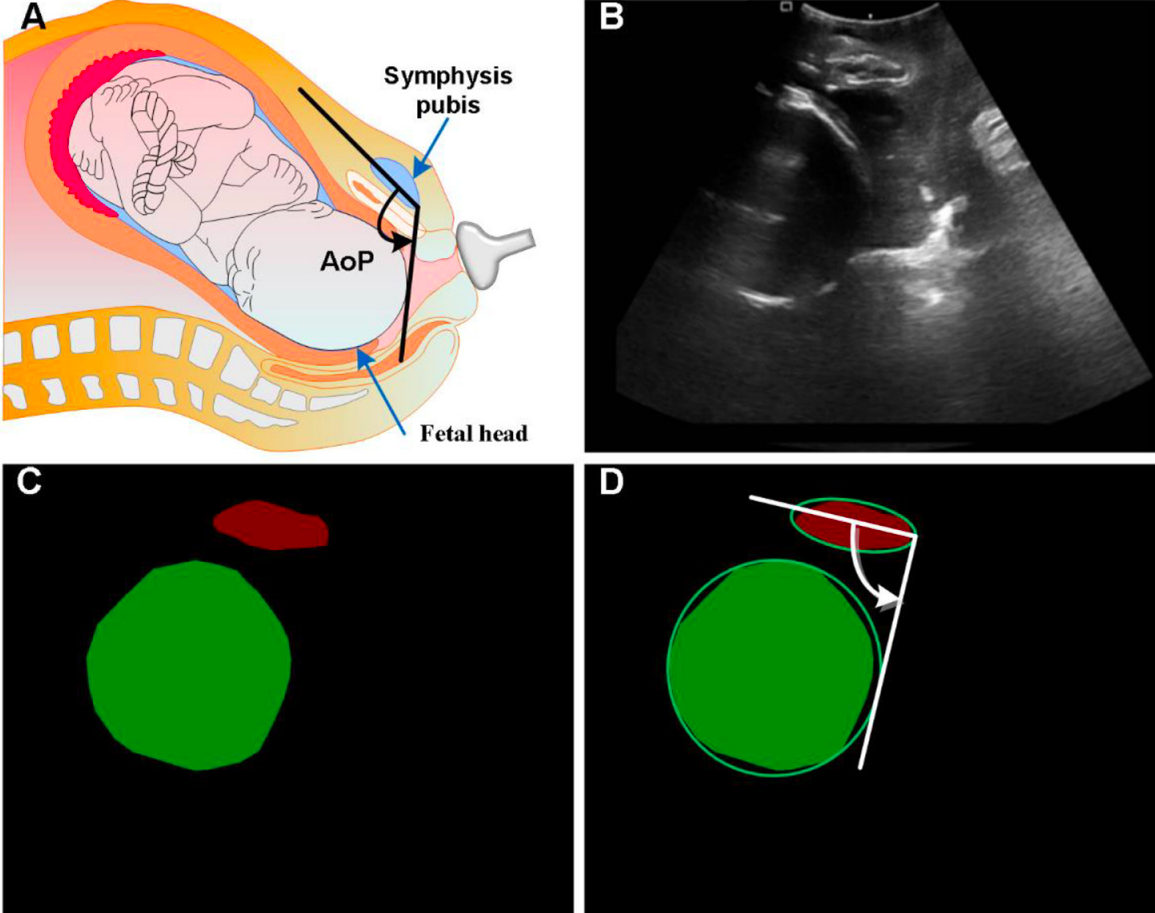
\includegraphics[width=\linewidth]{explanation}
        \vspace{-7mm}
        \caption{Assessment of FD in the birth canal by measurement AoP  ~\cite{LU2022107904}}
    \end{figure}
    \small
    \vspace{-5mm}
    \textbf{Data:}
    4000 MHA files for image data ($3\times256\times256$)
    and for labels ($256\times256$, pixels labeled as 
    0 - bg, 1 - PS, or 2 - FH).

    \textbf{Goal:}
    Segmentation algorithms, predicting images ($256\times256$) containing
    labeled pixels.


    \column{0.5\textwidth}
    \small
    \begin{itemize}
        \item \textit{Risk:} maternal and perinatal morbidity 
        \item \textit{Pathology:} longer labor duration 
        (slow progression of fetal descent(FD))
        \item \textit{Accurate assessment} of FD by 
        monitoring the FH station \textit{remains challenge} 
        in guiding obstetric management
        \item Manual segmentation of SP-FH from transperineal US (TPU)
        images is the most reliable, but \textit{extremely time-consuming} 
        \item Automatic measurement algorithms based on AI are 
        expected to be \textit{efficient, reproducible and objective} ~\cite{10.3389/fphys.2022.940150}
    \end{itemize}
    \end{columns}
\end{frame}


\section{Challenge Results}

%---------------------------------------------------------

\begin{frame}
    \frametitle{Metrics}
\vspace{-1.5em}
\normalsize
\resizebox{\textwidth}{!}{
\begin{tabular}{cccccccccccc}
\hline
Team           & AOP       & $HD_FH $   & $HD_PS$   & $ASD_FH$  & $ASD_PS$  & $HD_ALL$  & $ASD_ALL$ & $DICE_FH$ & $DICE_PS$ & $DICE_ALL$ & Score  \\
\hline
Gregor Koe     & 6.544     & 12.631    & 7.638   & 3.896   & 2.409   & 13.448   & 3.486   & 0.930   & ??      & 0.924    & 0.9418 \\
marwankefah    & 7.970     & 10.699    & 7.559   & 3.307  & 2.995   &12.059   &2.981     & 0.940 & ??      &0.935 & 0.9416 \\
Yaoyang Qiu    & 7.647     & 12.459    & 7.661   & 3.616   &2.257  & 13.615   & 3.238   & 0.936   & ??      & 0.930    & 0.939  \\
Gongping Chen  & 8.558     & 14.011    & 9.051   & 3.869   & 2.620   & 15.334   & 3.517   & 0.931   & 0.860   & 0.924    & 0.931  \\
Fangyijie Wang & 8.719     & 14.009    & 10.829  & 3.984   & 2.982   & 15.809   & 3.579   & 0.931   & 0.858   & 0.925    & 0.928  \\
Hongkun Sun   & 9.276     & 15.795    & 11.536  & 4.723   & 3.114   & 17.560   & 4.265   & 0.918   & 0.831   & 0.910    & 0.923  \\
Pengzhou Cai   & 12.199    & 20.031    & 14.068  & 7.099   & 4.208   & 21.873   & 6.058   & 0.879   & 0.804   & 0.872    & 0.897  \\
YuboTan        & 14.048    & 16.041    & 16.023  & 5.199   & 7.260   & 20.251   & 5.106   & 0.910   & ??      & 0.894    & 0.892  \\
\hline
\end{tabular}
}
    
\end{frame}


%---------------------------------------------------------
\begin{frame}
\begin{block}{Kitten's Remark}
    Sample text.
\end{block}
    
\begin{alertblock}{Feline's Important Theorem}
    Sample text in a charming red box.
\end{alertblock}
    
\begin{examples}
    Sample text in a paw-sitively green box. The title of the box is ``Kitten's Examples".
\end{examples}
\end{frame}

%---------------------------------------------------------
%Two columns
\begin{frame}
\frametitle{A Kitten's Two-column Slide}

\begin{columns}

\column{0.5\textwidth}
This is some text in the first column. Here's the famous equation: \myboxmath{E=mc^2}.

\begin{itemize}
\item First fluffy item
\item Second fluffy item
\end{itemize}

\column{0.5\textwidth}
In the second column, you'll find more purr-fection. This layout is as cute as a kitten's whiskers.
\end{columns}

\end{frame}



\begin{frame}
        \Large
        \begin{alertblock}{}
            \centering
            Thank you for your attention!
    
            Any questions?
        \end{alertblock}
\end{frame}

%---------------------------------------------------------

\section{References}

\begin{frame}
  \frametitle{References}
  \printbibliography % This command will generate the list of references
\end{frame}

\end{document}